\chapter{Uživatelské testování}

\section{System Usability Scale (SUS)}
System Usability Scale\footnote{\url{https://www.usability.gov/how-to-and-tools/methods/system-usability-scale.html}\nocite{SystemUsabilityScaleSUSUsabilitygov-2020-06-16}} je jednoduchý test na přívětivost uživatelského rozhraní aplikace. Cílem tohoto testování je seznámit uživatele s aplikací a pak mu položit 10 otázek, které SUS definuje. Na základě odpovědí na tyto otázky je pak spočteno skóre uživatelské přívětivosti. Aby testování bylo objektivní, je potřeba aplikaci testovat na osobách, jež se nepodílely na žádné části softwarového vývoje.

Testovaným osobám bude vysvětlen základní princip fungování aplikace a poté jim budou určeny jednoduché úkoly, které musí splnit. Znění těchto úkolů bude úmyslně napsáno velmi obecně a nebudou použity termíny, jež jsou použity v aplikaci. Testovaná osoba pak musí sama přijít na to, jak danou akci provést a díky tomu bude schopna objektivně zhodnotit přívětivost uživatelského rozhraní.

\begin{enumerate}
    \item Zjistěte, které taxony řadíme pod Vyšší rostliny (latinsky Embryophyta).
    \item Pokuste se vyrobit graf podobný grafu na obrázku. Toto uspořádání vrcholů do stromu se nazývá \textbf{dagre}. Konkrétní pořadí vrcholů není důležité. Místo ručního hledání Pteropsidy a moss se je pokuste vyhledat pomocí jejich názvu.
    \begin{figure}[h]
        \centering
        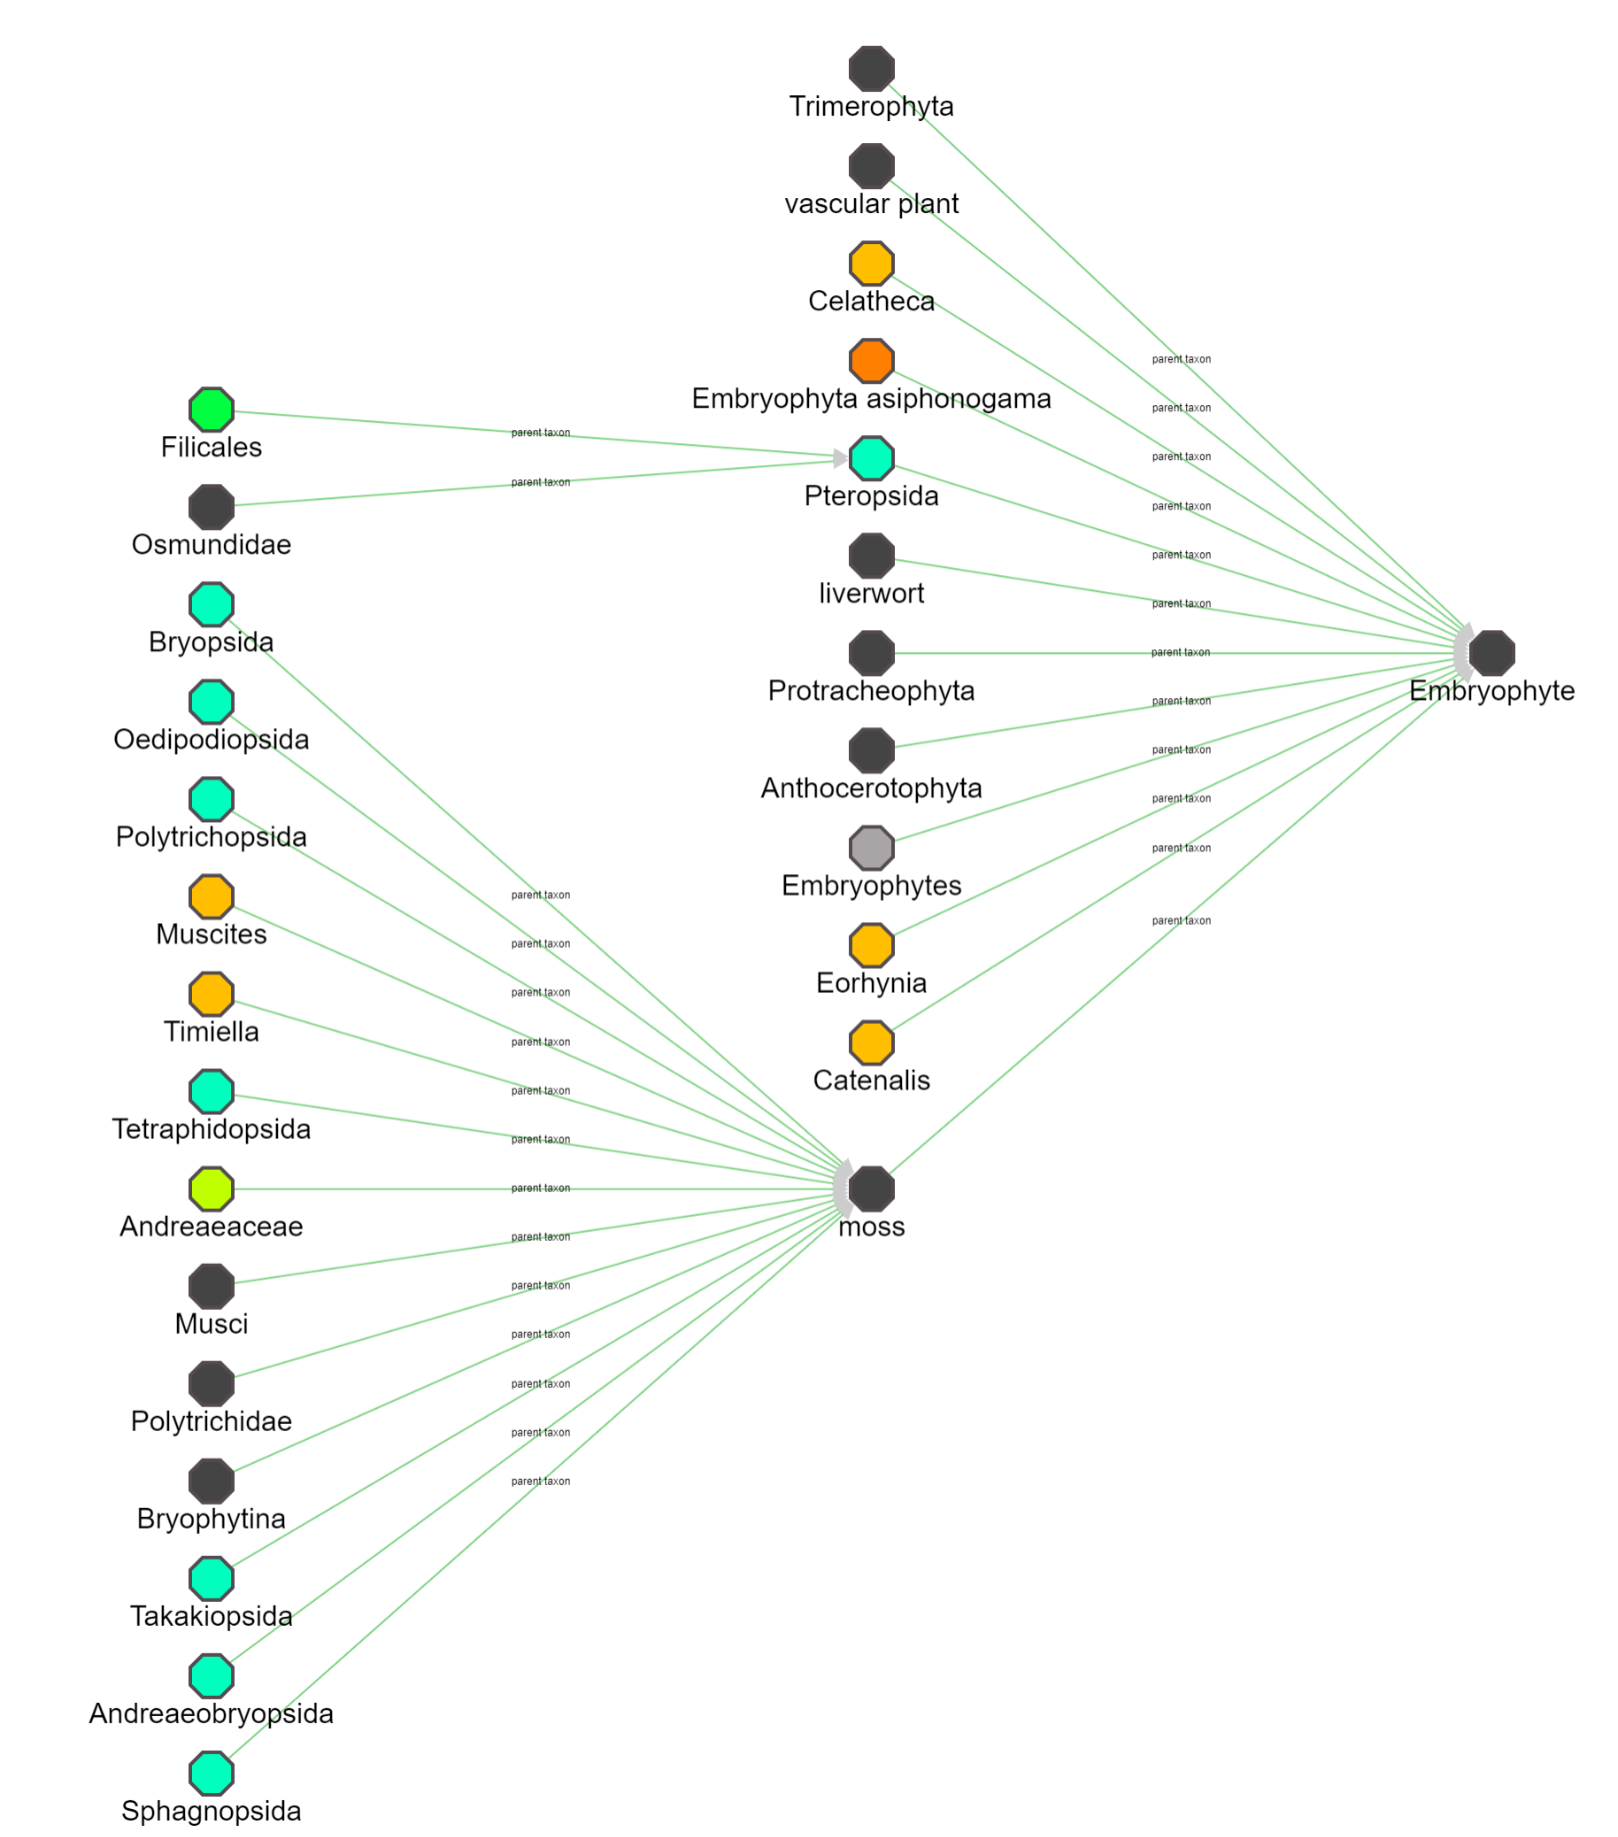
\includegraphics[width=0.5\textwidth]{media/sus-dagre.png}
    \end{figure}
    \item Stáhněte si aktuální graf do souboru, stránku aktualizujte a graf ze souboru opět načtěte.
    \item Nechte si zobrazit ze všech vrcholů jen ty, co mají třídu \uv{genus} (tedy chceme ty taxony, jež reprezentují rod).
    \item Odstraňte z grafu libovolný vrchol.
\end{enumerate}

\subsection{Výsledky testování SUS}

Na testování se podílelo celkem 13 respondentů. Níže je vypsán seznam deseti SUS otázek společně s výsledky testu.

Otázky mají určené pořadí a jsou formulovány tak, aby střídavě byla pozitivní odpověď \uv{soulasím} a \uv{nesouhlasím}. Na otázky se odpovídalo na stupnici 1-5.

\pgfplotstableread[row sep=\\,col sep=&]{
response & 1 & 2 & 3 & 4 & 5 & 6 & 7 & 8 & 9 & 10 \\
1        & 0 & 4 & 0 & 7 & 0 & 5 & 0 & 5 & 0 & 9  \\
2        & 1 & 5 & 2 & 3 & 2 & 5 & 0 & 4 & 3 & 3  \\
3        & 3 & 1 & 2 & 3 & 3 & 1 & 1 & 2 & 1 & 1  \\
4        & 6 & 3 & 7 & 0 & 3 & 2 & 8 & 2 & 4 & 0  \\
5        & 3 & 0 & 2 & 0 & 5 & 0 & 4 & 0 & 5 & 0 \\
}\dataone

\expandafter\def\csname question1\endcsname{Myslím, že bych chtěl tento systém často používat}
\expandafter\def\csname question2\endcsname{Systém mi přišel příliš složitý}
\expandafter\def\csname question3\endcsname{Systém mi přišel snadno použitelný}
\expandafter\def\csname question4\endcsname{K tomu, abych mohl(a) používat tento systém bych potřeboval(a) podporu technického personálu}
\expandafter\def\csname question5\endcsname{Přišlo mi, že různé funkce tohoto systému jsou dobře integrovány}
\expandafter\def\csname question6\endcsname{Přišlo mi, že je systém příliš nekonzistentní (rozdílné názvy pro stejné věci, rozdílné ovládání podobných prvků...)}
\expandafter\def\csname question7\endcsname{Myslím, že většina lidí by se naučila s tímto systémem zacházet velice rychle}
\expandafter\def\csname question8\endcsname{Systém mi přišel velice těžkopádný}
\expandafter\def\csname question9\endcsname{Při používání systému jsem se cítil(a) že vím co dělám}
\expandafter\def\csname question10\endcsname{Před použitím systému jsem se musel(a) naučit hodně věcí}
\newcommand\question[1]{\csname question#1\endcsname}

\bigskip

\noindent\foreach \x in {1,2,3,4,5,6,7,8,9,10}
{%
\begin{minipage}[]{0.45\textwidth}
\x. \question\x
\end{minipage}%
\begin{minipage}[]{0.05\textwidth}
\hfill
\end{minipage}%
\begin{minipage}[]{0.5\textwidth}
\begin{tikzpicture}
\selectcolormodel{gray}
    \begin{axis}[
            ybar,
            width=1\textwidth,
            height=0.5\textwidth,
            ytick style={draw=none},
            xtick style={draw=none},
            yticklabels={,,},
            nodes near coords,
            nodes near coords align={vertical},
            symbolic x coords={1,2,3,4,5},
            xtick=data,
            ymin=0,ymax=12,
            xticklabels={,,},
        ]
        \addplot table[x=response,y=\x]{\dataone};
    \end{axis}
\end{tikzpicture}\\
\vspace{-0.8cm}\\
\hspace*{0.2cm} Nesouhlasím\hfill Souhlasím\hspace*{1.4cm} \\
\end{minipage}\\
}

Na základě odpovědí na tyto otázky se pak počítá skóre následovně: Jednotlivé odpovědi u otázek se zprůměrují. Od každé liché otázky je odečtena $1$. (To jsou otázky, kde je pozitivní odpovědí \uv{souhlasím}, tedy $5$.) Pro každou sudou otázku pak její skóre bude odečteno od $5$. (U sudých otázek je pozitivní odpovědí \uv{nesouhlasím}, což odpovídá $1$.) Skóre všech otázek bude sečteno a vynásobeno $2,5$. Tak se získá celkové skóre v rozsahu $0$ až $100$.

Podle provedeného průzkumu SUS definuje, že průměrný systém s uživatelským rozhraním dosahuje skóre \textbf{68}.

Na základě výsledku testování pak vychází skóre této aplikace na \textbf{75,2}.

\bigskip

Respondenti také odpovídali na následující otázky
\begin{itemize}
    \item Víte, co je knowledge graph? - $75\%$ respondentů odpovědělo kladně.
    \item Víte, co jsou linked data? - $83\%$ respondentů odpovědělo kladně.
    \item Znáte SPARQL? - $50\%$ respondentů odpovědělo kladně.
\end{itemize}

\newpage


\section{Výsledky obecných otázek}
V rámci testování SUS byli respondenti navíc dotázáni, jaké části aplikace pro ně byly uživatelsky nepřívětivé a čemu neporozuměli. Výsledky jsou sepsány v následujícím seznamu společně s možným řešením.

\begin{itemize}
    \item Tlačítka v pravém dolním rohu grafové oblasti sloužící na obsluhu grafu (layoutování, zobrazení celého grafu, kompaktní mód) nejsou popsány a respondent odpověděl, že měl problém zjistit, co dělají.

    Tlačítkům bude vhodné přidat tooltipy vysvětlující jejich funkce obdobně, jak je tomu v jiných částech aplikace.
    \item Respondent nepochopil uživatelské rozhraní pro výběr layoutu. Neuvědomil si, že jednotlivé karty odpovídají konkrétním layoutům a vždy je aktivní pouze jeden layout. Měnil nastavení jiného layoutu, než toho, který byl aktivní.

    Zvážit kompletní změnu uživatelského rozhraní, které uživatele nutí nejprve zvolit layout a poté měnit jeho natavení.
    \item Respondent by ocenil, kdyby i levý panel s hlavním menu měl nápovědu s vysvětlivkami.
    \item Respondenti odpověděli, že nerozumí slovu \uv{layout}. Tuto funkci hledali pod \uv{možnosti pohledu}, což je nastavení pro \texttt{ViewOptions} popsané v kapitole \ref{komponenta-application}.

    Zvážit přejmenování layoutů a možností pohledů.
\end{itemize}

\section{Funkčnost aplikace}

Úkoly popsané v rámci SUS průzkumu sloužily také jako určitá forma uživatelského testování aplikace. I když nebylo jasně definováno, jak by aplikace měla na konkrétní úkoly reagovat, můžeme předpokládat, že úkoly proběhly úspěšně, neboť je všichni z respondentů dokončili.

Úkoly byly zadány tak, aby pokryly co nejvíce uživatelských požadavků popsaných v kapitole \ref{pozadavky-uzivatelske}.

Měřením code coverage bylo zjištěno, že provedením všech úkolů bylo pokryto \textbf{77\%} kódu. Většina aplikace tedy byla těmito úkoly úspěšně otestována.

Měření bylo prováděno s pomocí IDE WebStorm\footnote{\url{https://www.jetbrains.com/webstorm/}} od JetBrains pod prohlížečem Google Chrome. Během měření se postupně vykonaly všechny výše zmíněné úkoly nejjednodušším způsobem, jak lze daný úkol v aplikaci provést. Code coverage se měří z řádků zdrojového kódu, které byly v aplikaci spuštěny, přičemž se do výpočtu podílu nezahrnují komentáře, prázdné řádky a definice rozhraní, které se do JavaScriptu nepřekládají. Zbylých 23\% řádků pak odpovídá funkcím a větvím programu, které nebyly spuštěny.